% This is "sig-alternate.tex" V2.1 April 2013

\documentclass{sig-alternate-05-2015}


\begin{document}

\title{Interactive Model Serving for Regulatory Genomics}


\numberofauthors{4}

\author{
\alignauthor
Alyssa Morrow \\
       \email{akmorrow@berkeley.edu}
\alignauthor
Devin Petersohn \\
       \email{devin.petersohn@berkeley.edu}
\alignauthor Anthony Joseph \\
       \email{adj@berkeley.edu}
\and  % use '\and' if you need 'another row' of author names
\alignauthor Nir Yosef \\
       \email{nir.yosef@berkeley.edu}
}

\maketitle
\begin{abstract}
Current pipelines for training machine learning models on genomic and epigenetic datasets lack resources to scale to current datasets sizes. Furthermore, pipelines for testing and evaluating these machine learning models are segmented, as they require users to separately test pipelines and evaluate their methods using disjunct software. In this paper we survey current workflows for training, testing and evaluating genomic machine learning models and provide an alternative solution to connecting the dots between these processes. More specifically, present a complete fast and interactive pipeline that allows users to save prebuilt models and evaluate these models in a visual environment with low latency.
\end{abstract}


\printccsdesc

\keywords{Genomics; Model Serving; Transcription Factors}

\section{Introduction}
Regulatory genomics is a field of research that works to connect the function of DNA sequence, DNA interacting proteins and cell environment with gene expression. Understanding and predicting regulatory function is important, as it allows clinicians to predict the effect of an individual's genetic variants on their health and well being. Currently, there exist many different computational methods for prediction of regulatory function, including convolutional neural networks and SVM classification problems \cite{alipanahi2015predicting}, \cite{kelley2016basset}.  Datasets used to predict regulatory function are massive, reaching 15 TB in the ENCODE consortium \cite{encode2004encode}. However, these datasets are noisy, and thus analysis of regulatory predictions often require a human in the loop to visually interpret predictions against ground truth datasets produced in datasets such as ENCODE. \\


Current pipelines for training and analyzing predictive models for regulatory genomics include a segmented group of steps that are exclusive and require preprocessing between each stage. A schematic of this pipeline is shown in Figure~\ref{fig:strawmanPipeline}. In this state of the art pipeline, a user trains on local algorithm, such as a kernel method or neural network, built for a single machine. Because these methods are not built to scale past a single machine, users must first subselect regions of the genome to train on. After subselecting datapoints and training a model, a user would then subselect certain areas of the genome, and predict on these regions. Once the user has predicted on these regions, the user would then load these regions into a single node visualization tool, such as Integrated Genomics Viewer (IGV), and repeat this preprocessing step to validate their model \cite{igv2011}. \\

\begin{figure}
  \label{fig:strawmanPipeline}
  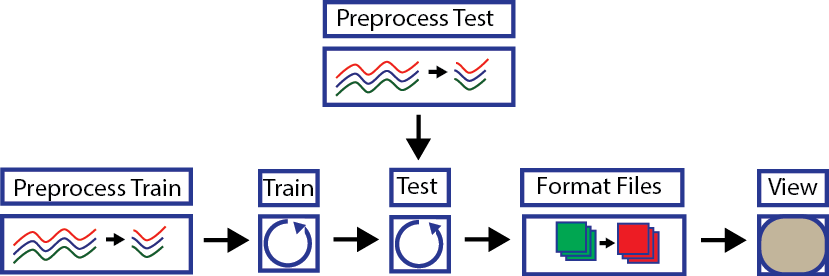
\includegraphics[width=0.5\textwidth]{figures/strawman.png}
  \caption{Stawman pipeline for training and evaluating model.}
\end{figure}

Here, we provide an end-to-end pipeline that efficiently computes and predicts on regulatory genomics while maintaining seamless integration between processing steps. In our previous work, we use a scalable and parallel algorithm to efficiently compute protein binding sites on the whole genome, bypassing user defined subselection methods required for local algorithms \cite{tfbinding}. Here, we utilize this algorithm to interactively predict on new datasets, and provide a full analysis pipeline to analyze results. Our pipeline allows users to interactively predict on regions of the genome, removing file preprocessing steps required in current pipelines. We compare our pipeline to the current state of the art approaches intended for a local machine, and then analyze pipeline latency at scale on the whole genome.

\section{Background}
In this section, we go through the current state of the are used for each portion in our pipeline. Pipeline stages discussed include predictive algorithms, and tools for evaluating models built from these algorithms.

\subsection{Algorithms}
Current algorithms for predicting on regulatory genomic datasets include neural networks and SVM classification. These methods train on small portions of the genome. For example, a neural net implementation DeepBind subselects 10,000 sequences to predict protein binding sites. Similarily, Kernel SVM uses 10,000 sequence to learn a classifier. Both tools are intended to run on a single machine. \\

\subsection{Evaluation Tools}
Main interative tools for evaluating algorithms discussed above include visualization tools, such as University of Santa Cruz Genome Browser and IGV (\cite{ucscbrowser}, \cite{igv2011}). IGV is a desktop application that allows visualization of a wide variety of genomic datasets. IGV is used by clinicians and researchers to verify anomalies in their data and verify predictions to original raw genomic datasets. IGV does not support integrated visualization of predictive models, so users attempting to perform visual analysis of models using heterogeneous datasets must predict outside of the visualization tool.

\section{Architecture}
In this section, we outline our design for an end-to-end machine learning pipeline on regulatory datasets. Our implementation builds upon previously built distributed genomics tools such as ADAM, Mango and Endive, which are described below. Finally, we will demonstrate how these tools can be connected to create an end-to-end pipeline for regulatory machine learning tasks. \\

\subsection{ADAM: Distributed Genomic Workloads}
ADAM is a framework for processing genomic data, and is built to run in the Spark ecosystem. ADAM uses distributed abstractions in Spark to batch process raw genomic datasets in parallel. More importantly, ADAM provides standardized schemas intended for various types of genomic datasets, presented in a narrow waist design that can be easily accessible by external applications. A figure of schema design is shown in Figure~\ref{fig:adam}. Important schemas that are used for regulatory datasets include Alignment Record, Features, and Variant schemas. We use these schemas to efficiently load and distribute regulatory datasets such as DNA sequence. Benefits of utilizing standardized schemas in a narrow waist schema allow users to transfer raw data and predictions across tools without having to parse files in a separate step.

\begin{figure}
  \label{fig:adam}
  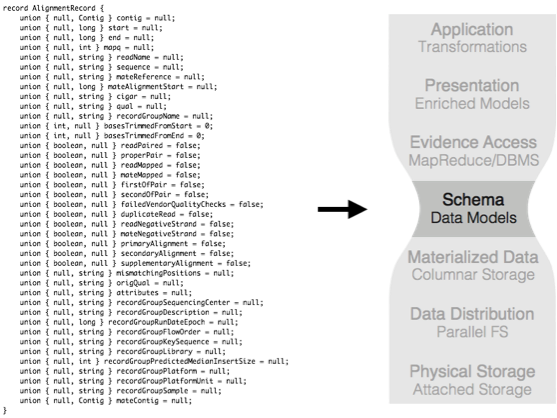
\includegraphics[width=0.5\textwidth]{figures/adamSchema.png}
  \caption{Example of AlignmentRecord schema used in
  Narrow waist design. Schema layer can be swapped in or
  Out for genomic workloads and sustituted in for legacy file formats.}
\end{figure}

\subsection{Mango: Genome Visualization}
Mango is a distributed genome visualization browser that selectively materializes and organizes genomic data to provide fast and fine grained queries on datasets. Mango materializes data from persistent storage as the user requests different regions of the genome. This data is efficiently partitioned and organized in memory using a specialized RDD structure built upon interval trees. This interval based organizational structure supports ad hoc queries, enabling exploratory interaction with genomic data.  Mango is built on top of Spark and ADAM. A demonstration of Mango architecture can be seen in Figure X. Mango is implemented in three layers, namely, the cluster, server and client. In the cluster layer, Mango is built on ADAM and Spark, allowing users to perform and visualize fine grained queries on large genomic files. The server layer reduces and samples queries so that users can visualize their queries in an efficient and interpretable manner.


\begin{figure}
  \label{fig:mango}
  
\includegraphics[width=0.5\textwidth]{figures/mango.png}
  \caption{Stack diagram for Mango architecture. Mango is built on ADAM and Spark, allowing users to perform and visualize fine grained queries on large genomic files.
  Endive}
\end{figure}

\subsection{Endive: Regulatory Machine Learning Abstractions}
Our machine learning tool, called Endive, provides core abstract stages for building end-to-end machine learning pipelines to train and evaluate on genomic datasets. These stages include data preprocessing, featurization, and various solvers apt for genomic workloads. These stages in a machine learning pipeline can be mixed and matched to create novel pipelines tailored to a genomic prediction task of interest.
Preprocessing in Endive involves taking raw genomic data and parsing it into a vector of numeric values which can be directly read by a machine learning model. These preprocessing steps include formatting datasets as well as joining together heterogeneous datasets into one record based on coordinate location in the genome.
Featurization steps in Endive involve taking preprocessed datasets created in the preprocessing stage and transforming these records to explicit features that can be trained and tested on. Table~\ref{table:featurization} contains examples of these featurization steps. These computed features can then be fed into a choice of solvers developed in Keystone ML to train these machine learning models \cite{keystone}.

\begin{table}
\centering
% \vspace{-0.4cm}
\caption{Example featurization steps available in Endive.}
\label{table:featurization}
% \hspace*{-0.96cm}
\begin{tabular}{|l|l|l|}
\hline
\textbf{Featurization Technique} & \textbf{Usage} \\
\hline
Read Wavelets (Raj et. al. 2015) & Identify patterns of \\ DNA-protein interaction \\ \hline
Kernel Approximations & Identification of  \\ protein binding sites \\ \hline
\end{tabular}
\end{table}


\begin{figure}
  \label{fig:pipeline}
  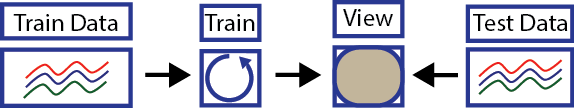
\includegraphics[width=0.5\textwidth]{figures/ourpipeline.png}
  \caption{Pipeline overview. We eliminate preprocessing and file formatting steps.}
\end{figure}


\section{Experiments}
For preliminary results, we train a model predicting protein binding sites using the kernel approximation featurization method described in Table~\ref{table:featurization}  from ENCODE datasets using DNA sequence. This model was solved using Keystone ML’s Weighted Least Squares estimator, which accounts for large class imbalance of positive binding sites across the genome. This model was trained both locally on a small dataset as well as in a distributed environment on a large (200 million) dataset. These models generated a 4 MB model to be tested on new datasets. This model was loaded into the Mango genome browser and was used to interactively predict on DNA reference sequences as the user scrolled to new regions of the browser.


\subsection{Local Comparison}
For a straw man comparison, we took the state of the art pipeline used to train and analyze protein binding sites on a local computer. We trained a model on 15,000 DNA sequences to predict the location of binding sites. These models were trained and tested on the EGR1 transcription factor. The strawman pipeline includes training a model with DeepBind, a neural net implementation to predict binding sites from DNA sequences \cite{alipanahi2015predicting}. To visualize results, we used IGV, a local genome browser.


Our pipeline trains a model on 15,000 sequences and uses Mango to analyze results. Because the models were too expensive to train locally, we train both straw man and our models on one machine with 24 Xeon processors, and 256 GB of ram and 1 Nvidia Tesla K20c GPU.

DEVIN TODO

\subsection{Whole Genome Prediction}
For our second experiment, we trained on the full genome, consisting of 200 million sequences to predict binding sites for protein EGR1. We visualize all raw data related to the model prediction problem, specifically DNA sequence and Dnase hypersensitivity files. Training the model took 58 minutes parallized across 16 nodes with Intel E5-2670 2.6 GHz 8 core CPU, 256 GB RAM and 4 1-TB HDFS hard drives. The generated model was saved and loaded into Mango to visualize predictions on raw datasets. Minimum, maximum and mean times to predict on new sequences using the sparcity model explained above is show in Table~\ref{table:fullGenome}. As in the local experiments, we test on region sizes of 2000 bp, 2000 bp, 4000bp, 8000bp and 16000bp. \\

The mean exectution time of 402.31 ms meets interactive requirements of 500ms. However, maximum execution time of 3.98s is too high for interactive time.

\begin{table}
\centering
% \vspace{-0.4cm}
\caption{Minimum, maximum and mean prediction response times for transcription factor EGR1.}
\label{table:fullGenome}
% \hspace*{-0.96cm}
\begin{tabular}{|l|l|l|}
\hline
\textbf{Min} & \textbf{Max} & \textbf{Mean} \\ \hline
3.09 ms & 3.98 s & 402.31 ms  \\ \hline
\end{tabular}
\end{table}

\section{Conclusion}
DEVIN TODO

\bibliographystyle{abbrv}
\bibliography{paperRef}  % sigproc.bib is the name of the Bibliography in this case




\end{document}
